\documentclass[crop,tikz]{standalone}
\usetikzlibrary{backgrounds}
\colorlet{blue}{cyan}
\tikzset{
  inverted/.style = {
    every path/.style = {draw=white,text=white},
    background rectangle/.style={fill},
    show background rectangle
  }
}

\tikzset{>=latex}
\usetikzlibrary{shapes}
\colorlet{gray}{gray!50}

\begin{document}
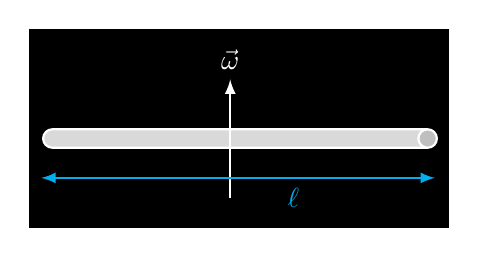
\begin{tikzpicture}[inverted,inverted]
  % cylinder
  \node (Z) at (0,0) [thick, cylinder, aspect=1, shape border rotate=0, draw, minimum height=5cm, minimum width=0.1cm, cylinder body fill=gray!60, cylinder uses custom fill, cylinder end fill=gray] {};
  % rotation axis
  \draw[->,thick] (0,-0.75) -- +(0,1.5) node[above] {$\vec{\omega}$};
  % radius
  \draw[<->,thick,blue] (-2.4,-0.5) -- node[below,xshift=2em] {$\ell$} +(5,0);
\end{tikzpicture}
\end{document}
